\section{Discussion}
\indent The T-test produced an outcome of P-value = 0.001524. The data shows the confidence level in the discernibility of aerial objects is 99.847\%. The data proved that the detection of an aerial biological from manmade vehicles is possible and could warrant further study and analysis using this and related techniques.
\indent The two data sets are normalized to prepare and clarify which type of T-test statistical analysis is needed for the data points. The normalized data shows that the variances are not matched and a heteroscedastic (different variabilities) one-tail T-test is needed. Observation of the normal distribution curve tells us that the mean of the data sets are different and a good candidate for the T-test analysis.\\  
\indent This study representing the initial work conducted with aerial morphology identification the default was chosen as it is universally accepted. A default significance level of 5\% was used. This study represents the initial work conducted with aerial morphology identification thus this was selected.\\
\indent The system's lower level process test, yielding the steady state profile confirms the theory of isolating the steady state portions of the aerial objects. The aerial biological profile experiences notable clipping around the wing tips during the ornithological motion the wings undergo. The steady state profile of the body of the aerial biological remains almost untouched as it is present in all motions that the aerial objects morphology.(As seen in Figure below)\\   
\begin{figure}[ht]
	\center 
	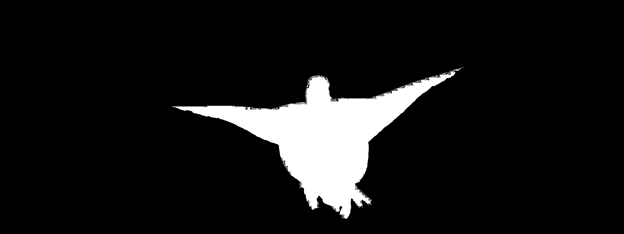
\includegraphics[height = 5cm]{Bird}
	\caption[Steady State Aerial Biological Profile]{Steady State Aerial Biological Profile from  Aerial Biological Video Sample: 4 (Left/Right Transient Wing Portions Clipped)}
\end{figure}
The steady state profile of an aerial manmade object also confirms the theoretical argument of the manmade aerial object and corresponding ratio maintaining the majority of its normal operating profile. As seen in figure below, the majority of the profile is complete confirming the steady state nature of manmade aerial objects, the small variations in the profile are due to transient portions as well as some noise experienced from the difference in position from one frame to the next.\\  
\begin{figure}[ht]
	\center 
	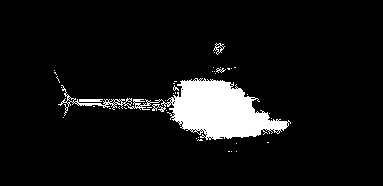
\includegraphics[height = 5cm]{Heli_Full}
	\caption[Steady State Aerial Manmade Object Profile]{Steady State Aerial Manmade Object Profile from Rotorcraft Video Sample: 2 (Steady State Portion Remains)}
\end{figure}
\indent Sources of errors in the study in respect to Boolean image multiplication include errors in position centering, thresholding. The ability of the system to keep the aerial object centered is essential to the boolean image multiplication process. The aerial object must overlay as cleanly as possible in order to yield the most accurate profile. The thresholding used in this study is a binary threshold that operates under a fixed value. Changes in lighting and object color may cause errors to occur. The reflectivity of the object due to sunlight and color of the object can be incorrectly transformed, which results in inaccurate aerial object profiles.  \\   
\indent The T-test analysis of the data sets resulted in a P-value = .001524. The P-value shows the probability that a random value will occur. The corresponding 99.847\% confidence level is found in the results. The P-value and the confidence level suggest that there is strong evidence against the null hypothesis, resulting in the rejection of the null hypothesis. The Alternative hypothesis is accepted.\\
\indent The statistical analysis T-test is a powerful statistical test. The problem with the T-test under the conditions that exist in the study are the quantity of the data. The T-test is said to require all points in studies under 15 data points to make a perfect normal distribution with no outliers. The T-test is less stringent for data sets of 40 and above, the test is said to be strong even when data is skewed beyond the distributed curve. The nonequivalent number of points in data sets are said to be valid, but the absent data points could represent the additional resolution of the data not seen otherwise. The absence of additional data points and resolution has the possibility to create a type I error of a false positive. \\ 
% This is where I left off (NEED POWER OF T TEST WITH SAMPLE SIZES)    
\indent The Alternative Hypothesis has been accepted and reveals the outcome of this study. The secondary question is if there is a bias threshold, can it be located and used to make the differentiation between the manmade aerial objects and the aerial biological objects. The mean values of the standard normal distributions previously calculated are used in the selection of the bias threshold. The calculated bias threshold was 30.41. In Table 3 and Table 4, bias threshold show that the bias threshold calculated using the average of the means found in the two data sets. The accuracy of the prediction based on the calculated bias threshold was 25\% and 50.3\%.\\ 
\indent The alternative hypothesis are the focus of this study, preliminary normal distributions of the individual video samples for the question of which frame and frame variation of the data most accurately represents the data. Normal distributions of each video sample data is collected not under any intense scrutiny, but as observation data and a courtesy to researchers continuing the study. Based on a snapshot of the data (See Appendix B), the time variation of my results in relation to the average, 73.53\% of the steady state ratio remained within a single standard deviation of the average. Further analysis is needed into the effects of time variation of frames on the steady state ratio.                               



